\documentclass{minimal}
\usepackage[utf8]{vietnam}
\usepackage{graphicx}
\usepackage{booktabs}
\usepackage{amsmath}
\usepackage{textpos}
\usepackage{pgfplots}
\usepackage{tikz}
\usepackage{hyperref}
\usepackage{caption}
\usetikzlibrary{shapes.geometric, arrows}
\usetikzlibrary {datavisualization} 
\pgfplotsset{compat=1.18, width = 7cm}
\usetikzlibrary{patterns}
\usepackage{algorithm}
\usepackage{color}
\usepackage{algorithmic}
\usepackage{footmisc}
\usepackage{indentfirst} 
\usepackage{comment}
\begin{document}

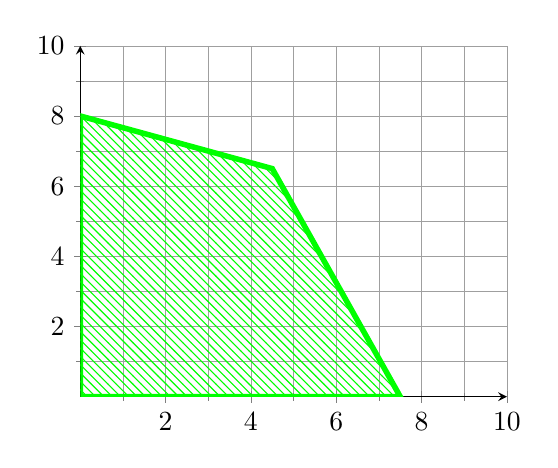
\begin{tikzpicture}
\begin{axis}
    [
    xmin=0,xmax=10,
    ymin=0,ymax=10,
    grid=both,
    grid style={line width=.1pt, draw=darkgray!50},
    major grid style={line width=.2pt,draw=darkgray!50},
    axis lines=middle,
    minor tick num=1,
    enlargelimits={abs=0},
    samples=100,
    domain = -20:20,
    ]
    \filldraw[green, pattern=north west lines, pattern color=green, line width=2pt] (0, 0) -- (0, 8) -- (4.5, 6.5) -- (7.5, 0) -- cycle;
\end{axis}
\end{tikzpicture}  
\end{document}